\documentclass[12pt]{article}
\linespread{1.25}
\usepackage{times}

\usepackage{pgfplots}
\pgfplotsset{compat = newest}
\usetikzlibrary{positioning, arrows.meta}
\usepgfplotslibrary{fillbetween}
\usepackage{amsmath}

\begin{document}

\begin{center}
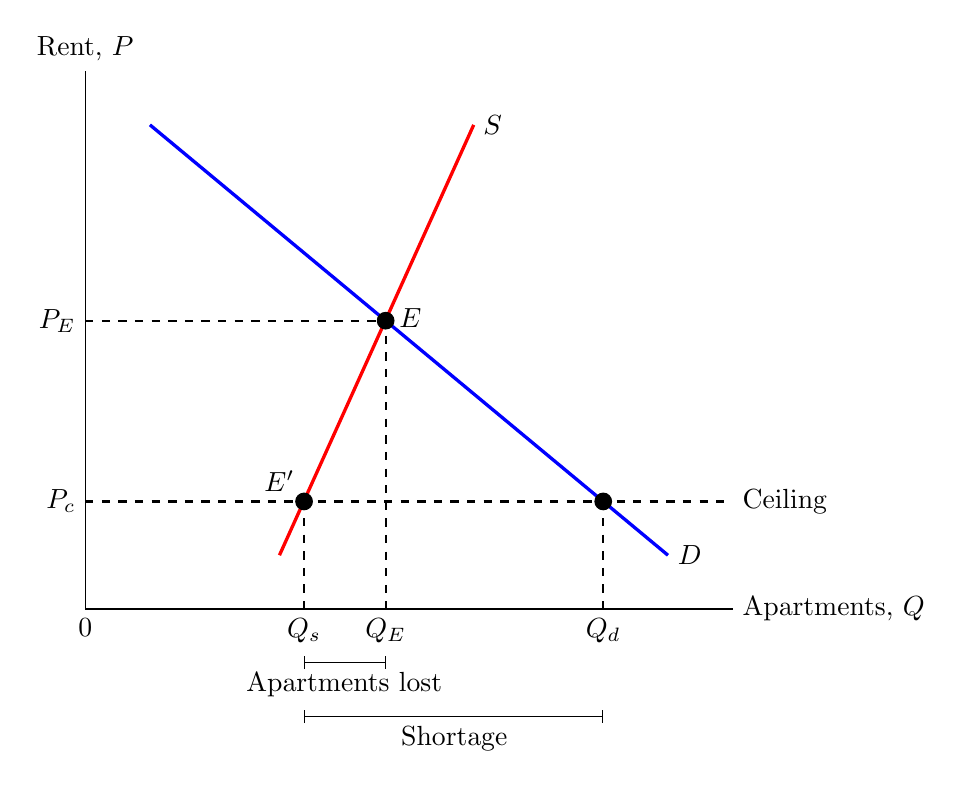
\begin{tikzpicture}
\begin{axis}[
    axis on top,
    scale=1.2,
    xmin=0, xmax=10,
    ymin=0, ymax=10,
    clip=false,
    axis lines*=left,
    xticklabels={,0},
    yticklabels={,,},
    tick style={draw=none},
    legend style={at={(1.25,0.9)},anchor=north east},
]

% Supply and Demand Curves
\addplot[color=blue, very thick] coordinates {(1,9)(9,1)};
\addplot[color=red, very thick] coordinates{(3,1)(6,9)};

% Quantity and Price Lines
\addplot[color=black, dashed, thick] coordinates {(0,5.36)(4.64,5.36)(4.64,0)};
\addplot[color=black, dashed, thick] coordinates {(0,2)(10,2)};
\addplot[color=black, dashed, thick] coordinates {(3.38,2)(3.38,0)};
\addplot[color=black, dashed, thick] coordinates {(8,2)(8,0)};

% Coordinate points
\addplot[color=black, mark=*, only marks, mark size=3pt] coordinates {(3.38,2)(4.64,5.36)(8,2)};

% Labels
\node [right] at (10, 2) {Ceiling};

\node [right] at (4.7,5.4) {$E$};
\node [above left] at (3.38,2) {$E^{\prime}$};

\node [above] at (current axis.above origin) {Rent, $P$};
\node [right] at (current axis.right of origin) {Apartments, $Q$};

\node [right] at (9,1) {$D$};
\node [right] at (6,9) {$S$};

\node [left] at (0, 5.36) {$P_E$};
\node [left] at (0, 2) {$P_c$};

\node [below] at (4.64, 0) {$Q_E$};
\node [below] at (3.38, 0) {$Q_s$};
\node [below] at (8, 0) {$Q_d$};

\draw[|-|] (3.38, -1) -- (4.64, -1);
\node [below] at (4, -1) {Apartments lost};
\draw[|-|] (3.38, -2) -- (8, -2);
\node [below] at (5.7, -2) {Shortage};
\end{axis}
\end{tikzpicture}
\end{center}
\textbf{Figure 8-1:} The effect of rent control on the rental market.

\end{document}